\subsubsection{無限のメモリの幻想を維持する}
以上紹介した構造では, リスト構造を表現することができるが,
メモリーが無限にあるという前提になってしまう. 実際の%
コンピュータでは, メモリが有限なので, メモリを使い切らない方法%
を考える必要がある. そのために, 使わなくなった結果などを消して%
そのメモリの部分を再利用できるようにする. その方法は
ガーベージコレクションという.

\paragraph{stop-and-copyガーベージコレクター}
ここで, \lstinline{root}というレジスターが%
現在アクセスできるすべてのデータの情報を持つ%
データ構造を指しているとする.

メモリで2つで分ける. 現在使っているデータは%
\lstinline{the-cars}と\lstinline{the-cdrs}とし,
使われていないメモリは\lstinline{new-cars}と\lstinline{new-cdrs}とする.

現在使っているメモリがいっぱいになると, 使っているデータのみ
使われていないメモリにコピーし, 現在のメモリをすべて空にする.

\begin{figure}[h]
  \centering
  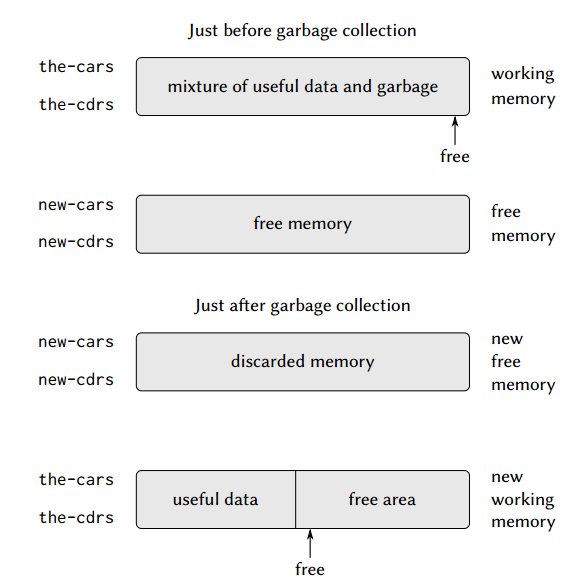
\includegraphics[height=6cm,width=8cm]{imgs/stop-and-copy.png}
\end{figure}
